\documentclass[../main.tex]{subfiles}

\begin{document}
\section{Conclusions} \label{sec:conclusions}
We have developed a non-metric calibration for light field acquisition, suitable for camera arrays, and flexible to viewing direction and planarity. The procedure is conceptually simple, yet demonstrates excellent results for light field applications, provided transform estimates are sufficiently accurate. Synthetic aperture focusing results compare well with other such setups (see figure~\ref{fig:occlusion-robustness-comparison}).

\begin{figure}[H]
    \centering
    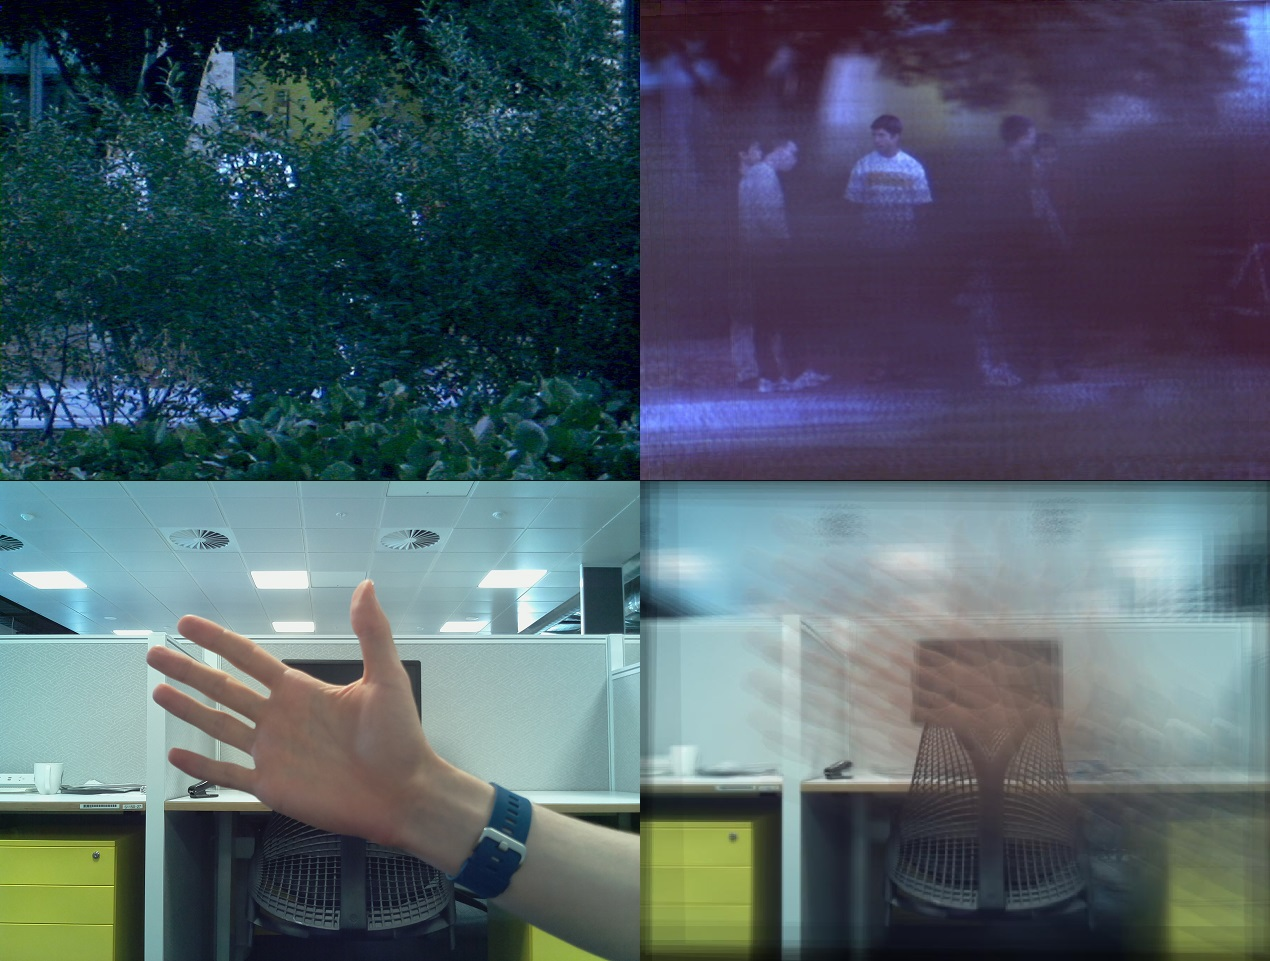
\includegraphics[width=\linewidth]{images/occlusion-robustness-comparison}
    \caption{Vaish et al's synthetic aperture focusing demonstration (top) and ours (bottom). The top images were adapted from \protect\bibentry{vaish2004using}}
    \label{fig:occlusion-robustness-comparison}
\end{figure}
\newpage

It is important to recognise that the calibration procedure is non-metric, thus there is no inherent baseline for a correct result or reprojection error. However, our calibration is also unique in that it is a non-metric calibration whose accuracy can be easily calculated to a fine degree, by measuring positional consistency of features on the reference plane. We have achieved such a positional consistency of 99.957\%.

The Raspberry Pi camera array is now significantly more capable as a light field camera, since camera poses are now retained by a new aluminium front-plate. Additionally, the camera array has demonstrated good performance with the new calibration procedure and synthetic aperture focusing applications. The camera array's potential for explorations in light field video has also been demonstrated, as synchronised capture and rendering of light field video has been achieved.

\end{document}